\chapter{रंग और प्रकाश-स्रोत}\label{ch:g11:color-light-sources}

किसी भौतिक विज्ञानी से टमाटर का रंग पूछिए और जवाब में सवाल मिलेगा: किस
प्रकाश में? टमाटर केवल उसी को \omterm{def:g11:color-light-sources:objectcolor}{विसरित} करता है जो उसे मिला है, लैंप
केवल वही देता है जो उसके \omterm{def:g10:light-spectra:white}{वर्णक्रम} में है, और आँख जो कुछ पहुँचता है
उसे तीन संख्याओं में निचोड़ देती है। रंग स्रोत, वस्तु और आँख के बीच का
समझौता है --- यह अध्याय तीनों पक्षों से बारी-बारी पूछताछ करता है।

\section{तीन संख्याओं में देखना}

\begin{definition}[शंकु कोशिकाएँ और त्रिवर्णी दृष्टि]\label{def:g11:color-light-sources:cones}
\omterm{def:g11:lenses-and-eye:eye}{दृष्टिपटल} (\cref{ch:g11:lenses-and-eye}) पर प्रकाश-संवेदी कोशिकाओं के दो कुल होते हैं:
\emph{शलाका कोशिकाएँ}\index{शलाका कोशिका}, जो मंद प्रकाश पर प्रतिक्रिया
करती हैं पर \omterm{def:g10:light-spectra:wavelength}{तरंगदैर्घ्य} की परवाह नहीं करतीं (रात की दृष्टि,
धूसर में), और \emph{शंकु कोशिकाएँ}\index{शंकु कोशिका}, जो तीन प्रकार की
होती हैं और $\qty{420}{nm}$ (नीला), $\qty{530}{nm}$ (हरा) तथा $\qty{560}{nm}$ (लाल) के पास सबसे
संवेदनशील रहती हैं। मनुष्य की रंग-दृष्टि
\emph{त्रिवर्णी}\index{त्रिवर्णी दृष्टि} है: \omterm{def:g10:light-spectra:white}{वर्णक्रम} चाहे जो
हो, मस्तिष्क को केवल तीन शंकु-प्रतिक्रियाएँ मिलती हैं, और रंग वही है जो
वह उस तिकड़ी से गढ़ लेता है।
\end{definition}

\begin{definition}[एक बोध के रूप में रंग]\label{def:g11:color-light-sources:perception}
इसलिए रंग एक \emph{बोध} है, अकेले प्रकाश का गुण नहीं: \omterm{def:g10:light-spectra:white}{वर्णक्रम}
हर \omterm{def:g10:light-spectra:wavelength}{तरंगदैर्घ्य} पर तीव्रता बताता है, जबकि आँख केवल तीन संख्याएँ
रखती है। जिन प्रकाशों के \omterm{def:g10:light-spectra:white}{वर्णक्रम} अलग हों पर तीनों शंकु
प्रतिक्रियाएँ एक जैसी हों, वे बिलकुल एक जैसे दिखते हैं: वे
\emph{समवर्णी}\index{समवर्णी} कहलाते हैं।
\end{definition}

\begin{example}[दो पीले]\label{ex:g11:color-light-sources:yellows}
सोडियम लैंप की $\qty{589}{nm}$ वाली रेखा लाल और हरी शंकु कोशिकाओं को लगभग
बराबर उत्तेजित करती है: मस्तिष्क कहता है \emph{पीला}। कोई परदा अपने लाल
($\qty{610}{nm}$) और हरे ($\qty{540}{nm}$) उप-पिक्सल जलाकर वही पीला दे देता है, और
$\qty{589}{nm}$ के पास कोई प्रकाश होता ही नहीं। प्रिज़्म दोनों को पलक झपकते अलग
कर देता है; आँख कभी नहीं कर पाती।
\end{example}

\section{प्रकाश जोड़ना}

\begin{definition}[योगात्मक संश्लेषण]\label{def:g11:color-light-sources:additive}
सफ़ेद परदे पर प्रकाश-पुंजों को एक के ऊपर एक डालने से उनके \omterm{def:g10:light-spectra:white}{वर्णक्रम} जुड़
जाते हैं: यही \emph{योगात्मक संश्लेषण}\index{योगात्मक संश्लेषण} है। तीन
सोच-समझकर चुने गए प्रकाश --- लाल, हरा और नीला, यानी \emph{योगात्मक
प्राथमिक रंग}\index{प्राथमिक रंग} --- मिलकर लगभग हर बोधगम्य रंग बना देते
हैं: R $+$ G $=$ पीला, R $+$ B $=$ मैजेंटा, G $+$ B $=$
सियान, और R $+$ G $+$ B $=$ सफ़ेद।
\end{definition}

\begin{proposition}[पूरक रंग]\label{prop:g11:color-light-sources:complementary}
जिन दो प्रकाशों का जोड़ सफ़ेद के रूप में बोधित हो, वे
\emph{पूरक}\index{पूरक रंग} कहलाते हैं। पीला/नीला, सियान/लाल और
मैजेंटा/हरा --- ये तीनों युग्म \omterm{prop:g11:color-light-sources:complementary}{पूरक} हैं।
\end{proposition}

\begin{proof}
पीला R $+$ G है; उसमें नीला जोड़ने से तिकड़ी पूरी होकर सफ़ेद बन जाती
है। बाक़ी दोनों युग्मों के लिए भी वही तर्क है, बस एक-एक \omterm{def:g11:color-light-sources:additive}{प्राथमिक रंग}
लेकर।
\end{proof}

\begin{example}[परदे]\label{ex:g11:color-light-sources:screen}
फ़ोन के परदे का हर पिक्सल तीन उप-पिक्सलों से बना है --- लाल, हरा, नीला,
हर एक $\qty{0.1}{mm}$ से भी पतला --- जो आँख के अलग कर पाने से कहीं अधिक पास हैं,
इसलिए उनके प्रकाश \omterm{def:g11:lenses-and-eye:eye}{दृष्टिपटल} पर ही जुड़ जाते हैं: पीले के लिए R
और G जलते हैं, नारंगी के लिए R पूरी शक्ति पर और G आधी पर, और
सफ़ेद के लिए तीनों। सफ़ेद हिस्से पर \omterm{def:g11:lenses-and-eye:magnifier}{आवर्धक} लगाइए और भेद खुल जाता है:
कहीं कोई सफ़ेद नहीं, बस R, G, B।
\end{example}

\begin{omfigure}
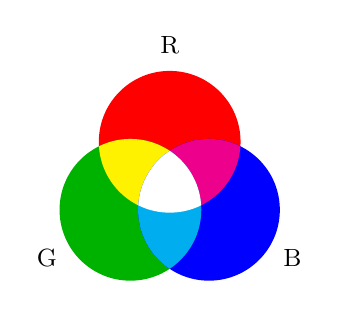
\begin{tikzpicture}[scale=0.72, font=\small]
  \fill[red] (90:0.8) circle (1.25);
  \fill[green!70!black] (210:0.8) circle (1.25);
  \fill[blue] (330:0.8) circle (1.25);
  \begin{scope}\clip (90:0.8) circle (1.25);\fill[yellow] (210:0.8) circle (1.25);\end{scope}
  \begin{scope}\clip (90:0.8) circle (1.25);\fill[magenta] (330:0.8) circle (1.25);\end{scope}
  \begin{scope}\clip (210:0.8) circle (1.25);\fill[cyan] (330:0.8) circle (1.25);\end{scope}
  \begin{scope}\clip (90:0.8) circle (1.25);\clip (210:0.8) circle (1.25);
    \fill[white] (330:0.8) circle (1.25);\end{scope}
  \node at (90:2.5) {R};\node at (210:2.5) {G};\node at (330:2.5) {B};
\end{tikzpicture}\qquad
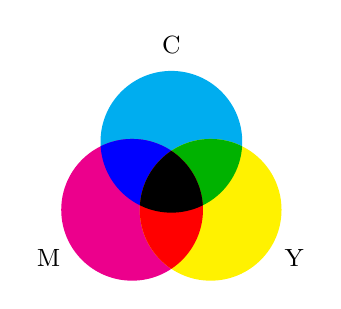
\begin{tikzpicture}[scale=0.72, font=\small]
  \fill[cyan] (90:0.8) circle (1.25);
  \fill[magenta] (210:0.8) circle (1.25);
  \fill[yellow] (330:0.8) circle (1.25);
  \begin{scope}\clip (90:0.8) circle (1.25);\fill[blue] (210:0.8) circle (1.25);\end{scope}
  \begin{scope}\clip (90:0.8) circle (1.25);\fill[green!70!black] (330:0.8) circle (1.25);\end{scope}
  \begin{scope}\clip (210:0.8) circle (1.25);\fill[red] (330:0.8) circle (1.25);\end{scope}
  \begin{scope}\clip (90:0.8) circle (1.25);\clip (210:0.8) circle (1.25);
    \fill[black] (330:0.8) circle (1.25);\end{scope}
  \node at (90:2.5) {C};\node at (210:2.5) {M};\node at (330:2.5) {Y};
\end{tikzpicture}

{\small एक-दूसरे पर पड़ते प्रकाश-पुंजों का \omterm{def:g11:color-light-sources:additive}{योगात्मक संश्लेषण}
(बाएँ) और \omterm{def:g10:light-spectra:white}{श्वेत प्रकाश} में एक के ऊपर एक रखे फ़िल्टरों का
\omterm{def:g11:color-light-sources:subtractive}{व्यवकलनात्मक संश्लेषण} (दाएँ)।}
\end{omfigure}

\section{श्वेत प्रकाश में से घटाना}

\begin{definition}[व्यवकलनात्मक संश्लेषण]\label{def:g11:color-light-sources:subtractive}
कोई \emph{फ़िल्टर}\index{फ़िल्टर} (रंगीन काँच, कोई जेल, स्याही या रंग की
परत) अपने पास आते \omterm{def:g10:light-spectra:white}{वर्णक्रम} का एक हिस्सा पार जाने देता है और बाक़ी
सोख लेता है। \omterm{def:g10:light-spectra:white}{श्वेत प्रकाश} में से पट्टियाँ \emph{हटाकर} रंग बनाना
\emph{व्यवकलनात्मक संश्लेषण}\index{व्यवकलनात्मक संश्लेषण} कहलाता है।
इसके \omterm{def:g11:color-light-sources:additive}{प्राथमिक रंग}, जो योगात्मक वालों के \omterm{prop:g11:color-light-sources:complementary}{पूरक} हैं, हर एक एक पट्टी घटाते
हैं: सियान $=$ सफ़ेद $-$ R, मैजेंटा $=$ सफ़ेद $-$ G, पीला
$=$ सफ़ेद $-$ B। एक के ऊपर एक रखे फ़िल्टर मिलकर घटाते हैं: सियान
$+$ पीला हरा छोड़ता है, सियान $+$ मैजेंटा नीला, मैजेंटा $+$ पीला
लाल, और तीनों मिलकर काला। छपाई और चित्रकारी इसी तरह चलती हैं, C, M, Y
स्याहियों से।
\end{definition}

\begin{method}[वर्णक्रम का हिसाब]\label{met:g11:color-light-sources:bookkeeping}
स्रोतों, फ़िल्टरों और वस्तुओं की किसी भी शृंखला से निकलने वाला
रंग बताने के लिए तीनों प्राथमिक पट्टियों का हिसाब रखिए: स्रोत के प्रकाश
को R, G, B की मात्रा के रूप में लिखिए; हर \omterm{def:g11:color-light-sources:subtractive}{फ़िल्टर} या सतह पर सोखी
गई पट्टियाँ काट दीजिए; और जो बचे उसका रंग बता दीजिए (कुछ न बचे $=$
काला)।
\end{method}

\begin{example}[फ़िल्टरों की एक शृंखला]\label{ex:g11:color-light-sources:chain}
\omterm{def:g10:light-spectra:white}{श्वेत प्रकाश} $(R, G, B)$ किसी पीले \omterm{def:g11:color-light-sources:subtractive}{फ़िल्टर} से गुज़रता है:
नीली पट्टी सोख ली जाती है और $(R, G)$ बचता है --- यानी पीला। फिर कोई सियान
\omterm{def:g11:color-light-sources:subtractive}{फ़िल्टर} लाल पट्टी सोख लेता है और $(G)$ बचता है: हरा।
फ़िल्टरों की जगह आपस में बदल दीजिए, कुछ नहीं बदलता: हर एक क्रम
की परवाह किए बिना अपनी ही पट्टी सोखता है।
\end{example}

\section{किसी वस्तु का रंग}

\begin{definition}[विसरण और वस्तु का रंग]\label{def:g11:color-light-sources:objectcolor}
कोई अपारदर्शी वस्तु अपने पास आते प्रकाश का एक हिस्सा सोख लेती है और
बाक़ी को \emph{विसरित}\index{विसरण} कर देती है --- यानी उसे हर दिशा में,
और उनमें हमारी आँखों की ओर भी, फिर से भेज देती है। \emph{किसी वस्तु का
रंग}\index{वस्तु का रंग} उस प्रकाश का रंग है जिसे वह \emph{दी गई रोशनी
में} विसरित करती है: वस्तु अपनी सोखने की आदतें देती है और स्रोत कच्चा
माल। लैंप बदलिए, रंग बदल जाएगा।
\end{definition}

\begin{example}[लाल कमीज़]\label{ex:g11:color-light-sources:redshirt}
कोई कमीज़ दिन के उजाले में लाल दिखती है: वह हरी और नीली पट्टियाँ सोख
लेती है और लाल को \omterm{def:g11:color-light-sources:objectcolor}{विसरित} कर देती है। शुद्ध हरे प्रकाश में
\omterm{def:g11:color-light-sources:objectcolor}{विसरित} करने को लाल पट्टी है ही नहीं: कमीज़ सब कुछ सोख लेती है और काली
दिखती है। मैजेंटा प्रकाश $(R, B)$ में वह अकेली लाल पट्टी \omterm{def:g11:color-light-sources:objectcolor}{विसरित}
करती है: फिर भी लाल। कोई सफ़ेद वस्तु अपने पास आती हर पट्टी \omterm{def:g11:color-light-sources:objectcolor}{विसरित}
कर देती है (हरे प्रकाश में वह हरी दिखती है); और कोई काली वस्तु हर प्रकाश
में सब सोख लेती है --- यही कारण है कि काले कपड़े धूप में गरम हो जाते हैं।
\end{example}

\begin{omfigure}
\begin{tikzpicture}[scale=0.9, font=\small]
  \fill[red!80] (0,0) rectangle (1.6,1.0);
  \node at (0.8,0.5) {कमीज़};
  \draw[-Stealth, red, thick] (-1.9,1.45) -- (-0.1,0.9);
  \draw[-Stealth, green!65!black, thick] (-1.9,0.95) -- (-0.1,0.62);
  \draw[-Stealth, blue, thick] (-1.9,0.45) -- (-0.1,0.34);
  \draw[-Stealth, red, very thick] (1.7,0.9) -- (3.1,1.45)
    node[above right=-3pt] {लाल विसरित};
  \node[anchor=west] at (1.7,0.3) {G, B सोखे गए};
  \node at (0.8,-0.55) {श्वेत प्रकाश: लाल कमीज़};
\end{tikzpicture}\qquad
\begin{tikzpicture}[scale=0.9, font=\small]
  \fill[black!85] (0,0) rectangle (1.6,1.0);
  \node[white] at (0.8,0.5) {कमीज़};
  \draw[-Stealth, green!65!black, thick] (-1.9,0.95) -- (-0.1,0.62);
  \node[anchor=west] at (1.7,0.75) {कुछ विसरित नहीं};
  \node[anchor=west] at (1.7,0.3) {G सोखा गया};
  \node at (0.8,-0.55) {हरा प्रकाश: काली कमीज़};
\end{tikzpicture}

{\small वही लाल कमीज़, दो रोशनियों में: वह केवल लाल पट्टी \omterm{def:g11:color-light-sources:objectcolor}{विसरित} कर सकती
है --- जो \omterm{def:g10:light-spectra:white}{श्वेत प्रकाश} में मौजूद है और हरे प्रकाश में ग़ायब।}
\end{omfigure}

\section{प्रकाश-स्रोत और वर्ण ताप}

\begin{definition}[तापदीप्त स्रोत]\label{def:g11:color-light-sources:incandescent}
जो स्रोत गरम होने के कारण दमके --- लौ, तंतु, तारा --- वह
\emph{तापदीप्ति}\index{तापदीप्ति} से चमकता है। उसका \omterm{def:g10:light-spectra:white}{वर्णक्रम}
\cref{ch:g10:light-spectra} वाला सतत तापीय \omterm{def:g10:light-spectra:white}{वर्णक्रम} होता है, और उसका शिखर वीन का नियम
(\cref{prop:g10:light-spectra:wien}) मानता है,
\[
\lambda_{\max} \times T = \qty{2.90e-3}{m.K},
\]
और अब से यही हमारा संख्यात्मक औज़ार है: शिखर नापिए, ताप हाज़िर।
\end{definition}

\begin{example}[एक बेहद अदक्ष लैंप]\label{ex:g11:color-light-sources:bulb}
$T = \qty{2700}{K}$ पर चलते टंगस्टन तंतु का शिखर $\lambda_{\max} = \qty{2.90e-3}{m.K}/\qty{2700}{K} = \qty{1.07e-6}{m}
= \qty{1070}{nm}$ पर पड़ता है, यानी गहरे
\omterm{def:g10:light-spectra:wavelength}{अवरक्त} में: अधिकांश विद्युत शक्ति अदृश्य विकिरण बनकर निकल
जाती है और केवल लगभग $5\%$ प्रकाश बनता है --- तापदीप्त बल्ब मुख्यतः एक
हीटर ही था।
\end{example}

\begin{omfigure}
\begin{tikzpicture}
\begin{axis}[omaxis, width=9.4cm, height=5.4cm,
    xlabel={$\lambda$ (nm)}, ylabel={तीव्रता (मनमाने मात्रक)},
    xmin=0, xmax=2400, ymin=0, ymax=10,
    xtick={400, 800, 1200, 1600, 2000}, ytick=\empty]
  \fill[gray, opacity=0.12] (axis cs:400,0) rectangle (axis cs:800,10);
  \node[gray, anchor=south] at (axis cs:600,8.7) {दृश्य};
  \addplot[omThm, thick, domain=200:2300, samples=160]
    {3.2e16 * x^(-5) / (exp(2400/x) - 1)};
  \addplot[omDef, thick, domain=250:2300, samples=160]
    {3.84e17 * x^(-5) / (exp(4800/x) - 1)};
  \draw[dashed, omThm] (axis cs:483,0) -- (axis cs:483,8.5);
  \draw[dashed, omDef] (axis cs:967,0) -- (axis cs:967,3.2);
  \node[omThm, anchor=west] at (axis cs:520,9.0) {$\qty{6000}{K}$};
  \node[omDef, anchor=west] at (axis cs:1010,3.4) {$\qty{3000}{K}$ ($\times 12$)};
\end{axis}
\end{tikzpicture}

{\small $\qty{6000}{K}$ और $\qty{3000}{K}$ पर तापीय \omterm{def:g10:light-spectra:white}{वर्णक्रम}, और $483$ तथा $\qty{967}{nm}$ पर
बिंदुदार शिखर $\lambda_{\max}$; ठंडी वाली वक्र को बारह गुना बढ़ाकर न दिखाया जाता
तो वह अक्ष से चिपकी रह जाती।}
\end{omfigure}

\begin{definition}[वर्णक्रमी लैंप और लेज़र]\label{def:g11:color-light-sources:lamps}
\emph{वर्णक्रमी लैंप}\index{वर्णक्रमी लैंप} --- यानी विसर्जन से उत्तेजित
कोई कम दाब वाली गैस: सोडियम, पारा, नियॉन --- \omterm{def:g10:light-spectra:emission}{रेखा
वर्णक्रम} (\cref{ch:g10:light-spectra}) देता है: कुछ अलग-थलग \omterm{def:g10:light-spectra:wavelength}{तरंगदैर्घ्य}, और बीच में
कुछ नहीं। \emph{लेज़र}\index{लेज़र} इससे भी आगे जाता है: एक ही
\omterm{def:g10:light-spectra:wavelength}{तरंगदैर्घ्य}, \omterm{def:g10:light-spectra:white}{एकवर्णी प्रकाश}, और वह भी एक \omterm{def:g11:lenses-and-eye:lens}{पतले} पुंज में।
\end{definition}

\begin{definition}[LED]\label{def:g11:color-light-sources:led}
\emph{प्रकाश-उत्सर्जक डायोड}\index{प्रकाश-उत्सर्जक डायोड} (LED) कुछ दसियों
नैनोमीटर चौड़ी एक \emph{लगभग एकवर्णी}\index{लगभग एकवर्णी} पट्टी
उत्सर्जित करता है: इतनी सँकरी कि रंग निश्चित लगे, पर \omterm{def:g11:color-light-sources:lamps}{लेज़र} की
रेखा से कहीं चौड़ी। सफ़ेद LED असल में एक नीला LED (शिखर $\qty{450}{nm}$ के पास)
होता है जिस पर \emph{स्फुरदीप्त पदार्थ}\index{स्फुरदीप्त पदार्थ} की परत
चढ़ी होती है, जो नीले का एक हिस्सा सोखकर उसे एक चौड़ी पीली पट्टी के रूप
में फिर उत्सर्जित करती है: और चूँकि नीला तथा पीला \omterm{prop:g11:color-light-sources:complementary}{पूरक} हैं (\cref{prop:g11:color-light-sources:complementary}),
मिश्रण सफ़ेद पढ़ा जाता है।
\end{definition}

\begin{definition}[वर्ण ताप]\label{def:g11:color-light-sources:colortemp}
किसी सफ़ेद-से दिखते स्रोत का \emph{वर्ण ताप}\index{वर्ण ताप} उस तापदीप्त
पिंड का ताप है जिसकी रंगत से उसके प्रकाश की रंगत मेल खाती है: मोमबत्ती
$\qty{1800}{K}$, तापदीप्त बल्ब $\qty{2700}{K}$, हैलोजन $\qty{3400}{K}$, दोपहर का सूर्य $\qty{5500}{K}$,
बादल भरा दिन का उजाला $\qty{6500}{K}$। यह रंग का लेबल है, थर्मामीटर का पाठ नहीं
--- $\qty{6500}{K}$ वाला LED कमरे के ताप पर ही चलता है --- और शब्दावली उलटी चलती
है: कम वर्ण ताप ``गरम'' नारंगी पढ़ा जाता है और अधिक ``ठंडा'' नीलापन लिए।
\end{definition}

\begin{omfigure}
\begin{tikzpicture}[font=\small]
  \shade[left color=orange!95!red, right color=white] (0,0) rectangle (5.4,0.7);
  \shade[left color=white, right color=blue!25] (5.4,0) rectangle (9,0.7);
  \draw (0,0) rectangle (9,0.7);
  \draw[-Stealth] (0,-0.5) -- (9.6,-0.5)
    node[right] {वर्ण ताप (K)};
  \foreach \x/\l in {0.5/1800, 2.0/2700, 3.1/3400, 6.5/5500, 8.2/6500}
    \draw (\x,-0.4) -- (\x,-0.6) node[below] {\l};
  \foreach \x/\n in {0.5/candle, 2.0/bulb, 3.1/halogen, 6.5/sun,
      8.2/overcast}
    \node[above] at (\x,0.7) {\n};
\end{tikzpicture}

{\small आम स्रोतों का वर्ण-ताप पैमाना: ``गरम'' नारंगी रंगतें कम $T$
पर बैठती हैं और ``ठंडी'' नीली रंगतें अधिक $T$ पर।}
\end{omfigure}

\section{अभ्यास}

\begin{exercise}[$\star$]\label{exo:g11:color-light-sources:1}
बताइए कि सफ़ेद परदे पर एक साथ ये पड़ें तो कौन-सा रंग बोधित होगा: (क) लाल
और हरा प्रकाश; (ख) हरा और नीला प्रकाश; (ग) तीनों \omterm{def:g11:color-light-sources:additive}{प्राथमिक रंग}। नीले का
\omterm{prop:g11:color-light-sources:complementary}{पूरक} कौन-सा प्रकाश है?
\end{exercise}

\begin{exercise}[$\star$]\label{exo:g11:color-light-sources:2}
कोई परदा ये दिखाने के लिए कौन-से उप-पिक्सल (R, G, B) जलाता है: पीला,
मैजेंटा, सफ़ेद, काला, नारंगी?
\end{exercise}

\begin{exercise}[$\star$]\label{exo:g11:color-light-sources:3}
\omterm{def:g10:light-spectra:white}{श्वेत प्रकाश} किसी मैजेंटा \omterm{def:g11:color-light-sources:subtractive}{फ़िल्टर} से गुज़रता है। कौन-सी
पट्टी सोखी जाती है और कौन-सा रंग निकलता है? फिर उसके पीछे एक सियान
\omterm{def:g11:color-light-sources:subtractive}{फ़िल्टर} भी लगा दिया जाता है: अब क्या निकलता है?
\end{exercise}

\begin{exercise}[$\star$]\label{exo:g11:color-light-sources:4}
\omterm{def:g10:light-spectra:white}{श्वेत प्रकाश} में किसी झंडे की एक पट्टी पीली दिखती है। वह कौन-सी
पट्टियाँ \omterm{def:g11:color-light-sources:objectcolor}{विसरित} करती है और कौन-सी सोखती है? (क) लाल और (ख) नीले प्रकाश
में उसका रंग?
\end{exercise}

\begin{exercise}[$\star$]\label{exo:g11:color-light-sources:5}
किसी तारे के \omterm{def:g10:light-spectra:continuous}{सतत वर्णक्रम} का शिखर $\lambda_{\max} = \qty{580}{nm}$ पर है। उसकी सतह का
ताप निकालिए।
\end{exercise}

\begin{exercise}[$\star\star$]\label{exo:g11:color-light-sources:6}
मोमबत्ती की लौ लगभग $\qty{1800}{K}$ पर होती है। (क) $\lambda_{\max}$ निकालिए और उसका
क्षेत्र बताइए। (ख) फिर भी लौ नारंगी दिखती है: समझाइए।
\end{exercise}

\begin{exercise}[$\star\star$]\label{exo:g11:color-light-sources:7}
कोई साइकिल सवार लाल जैकेट और सियान दस्ताने पहने है। \cref{met:g11:color-light-sources:bookkeeping} की सहायता से
हर चीज़ का \omterm{def:g11:lenses-and-eye:images}{आभासी} रंग बताइए, (क) \omterm{def:g10:light-spectra:white}{श्वेत प्रकाश} में; (ख) लाल प्रकाश
में; (ग) हरे प्रकाश में।
\end{exercise}

\begin{exercise}[$\star\star$]\label{exo:g11:color-light-sources:8}
कोई पुरानी गली कम दाब वाले सोडियम लैंपों से रोशन है ($\qty{589}{nm}$
पर एक ही रेखा)। (क) यह किस तरह का \omterm{def:g10:light-spectra:white}{वर्णक्रम} है, और उसके नीचे
\emph{कोई भी} वस्तु कौन-से रंग ले सकती है? (ख) कोई कार उन लैंपों के नीचे
काली दिखती है और दिन के उजाले में नीली: समझाइए।
\end{exercise}

\begin{exercise}[$\star\star$]\label{exo:g11:color-light-sources:9}
कोई हरा \omterm{def:g11:color-light-sources:lamps}{लेज़र} सूचक $\qty{532}{nm}$ पर उत्सर्जन करता है। (क) उसका पुंज
किसी प्रिज़्म से गुज़रता है: नतीजे की तुलना सफ़ेद पुंज वाले नतीजे से
कीजिए, और दिखाए गए गुण का नाम बताइए। (ख) फिर वह किसी लाल
\omterm{def:g11:color-light-sources:subtractive}{फ़िल्टर} से मिलता है: क्या बाहर निकलता है?
\end{exercise}

\begin{exercise}[$\star\star$]\label{exo:g11:color-light-sources:10}
सफ़ेद LED (नीला डायोड और \omterm{def:g11:color-light-sources:led}{स्फुरदीप्त पदार्थ}) का \omterm{def:g10:light-spectra:white}{वर्णक्रम}
बताइए, और समझाइए कि उसका प्रकाश सफ़ेद क्यों बोधित होता है। कोई गहरी लाल
वस्तु सस्ते सफ़ेद LED के नीचे दिन के उजाले की तुलना में फीकी क्यों दिखती
है?
\end{exercise}

\begin{exercise}[$\star\star$]\label{exo:g11:color-light-sources:11}
तापदीप्त पिंड के लिए $\lambda_{\max}$ निकालिए, (क) मोमबत्ती के \omterm{def:g11:color-light-sources:colortemp}{वर्ण ताप}
($\qty{1800}{K}$) पर; (ख) बादल भरे दिन के उजाले के ($\qty{6500}{K}$) पर। उन दोनों
प्रकाशों में से किसे ``गरम'' कहा जाता है? टिप्पणी कीजिए।
\end{exercise}

\begin{exercise}[$\star\star\star$]\label{exo:g11:color-light-sources:12}
कोई सोडियम लैंप ($\qty{589}{nm}$) और पीला दिखाता कोई परदा (उप-पिक्सल $\qty{610}{nm}$ और
$\qty{540}{nm}$ पर) बिलकुल एक ही रंग के दिखते हैं। (क) ऐसे दो प्रकाशों को क्या
कहते हैं, और उनका होना रंग के बारे में क्या सिद्ध करता है? (ख) उन्हें
अलग बताने वाले दो अलग-अलग प्रयोग सुझाइए, और हर एक का नतीजा भी बताइए।
\end{exercise}

\begin{exercise}[$\star\star\star$]\label{exo:g11:color-light-sources:13}
रंगमंच का कोई हैलोजन स्पॉट $\qty{3200}{K}$ पर चलता है। (क) $\lambda_{\max}$ निकालिए: यह
प्रकाश दिन के उजाले से अधिक गरम है या अधिक ठंडा? (ख) दिन के उजाले की
नक़ल करने के लिए स्पॉट पर हल्के नीले जेल की परत चढ़ाई जाती है। जेल क्या
हटाता है, और मंच मंद क्यों पड़ जाता है? (ग) समझाइए कि कोई जेल इसके बजाय
स्पॉट के \omterm{def:g10:light-spectra:white}{वर्णक्रम} के नीले सिरे को \emph{बढ़ा} क्यों नहीं सकता।
\end{exercise}

\begin{exercise}[$\star\star\star$]\label{exo:g11:color-light-sources:14}
कोई क़साई अपने माँस की दुकान को $\qty{2700}{K}$ \omterm{def:g11:color-light-sources:colortemp}{वर्ण ताप} वाले LED से
रोशन करता है; बग़ल वाला मछली बेचने वाला $\qty{6500}{K}$ काम में लेता है। (क) दोनों में से हर
रोशनी की रंगत और लाल माँस तथा सफ़ेद मछली पर उसका असर बताइए। (ख) क्या
इनमें से किसी दुकानदार ने अपना माल बदला है? ठीक-ठीक बताइए कि बदलाव कहाँ
हो रहा है (\cref{def:g11:color-light-sources:objectcolor})।
\end{exercise}

\begin{exercise}[$\star\star\star$]\label{exo:g11:color-light-sources:15}
किसी वेधशाला के बग़ल का शहर अपनी सड़कें फिर से रोशन करना चाहता है और
कम दाब वाले सोडियम लैंपों तथा चौड़े \omterm{def:g10:light-spectra:white}{वर्णक्रम} वाले सफ़ेद
LED के बीच झूल रहा है। (क) खगोलविद कौन-सा चुनाव पसंद करेंगे, और क्यों?
(सोचिए कि एक अकेला \omterm{def:g11:color-light-sources:subtractive}{फ़िल्टर} उनके चित्रों में से क्या हटा सकता
है।) (ख) चालक और पैदल चलने वाले कौन-सा पसंद करेंगे? वस्तुओं के रंगों से
उचित ठहराइए। (ग) \omterm{def:g11:color-light-sources:colortemp}{वर्ण ताप} की भाषा में कोई बीच का रास्ता सुझाइए।
\end{exercise}

\section{समस्या: रंग की इंजीनियरी}

\begin{problem}[{सप्ताहांत समस्या --- मंच की रोशनी, सोडियम वाली सड़कें
और सफ़ेद LED: रंग गढ़ा कैसे जाता है, तीन स्पॉटलाइटों से जो कोई भी रंगत
रंग सकते हैं, उस चिप तक जो यह पन्ना रोशन करती है}]
\label{pb:g11:color-light-sources:1}
किसी प्रकाश-सज्जाकार के पास केवल लाल, हरा और नीला स्पॉटलाइट हैं; किसी
सड़क-अभियंता के पास ऐसा लैंप है जो एक ही \omterm{def:g10:light-spectra:wavelength}{तरंगदैर्घ्य} देता है; और
किसी चिप बनाने वाले के पास ऐसा डायोड है जो केवल नीला चमकता है। तीनों रंग
बेचते हैं। यह समस्या बारी-बारी उनके पेशे चलाती है --- मंच पर योगात्मक
मिश्रण, सड़क पर \omterm{def:g10:light-spectra:white}{एकवर्णी} मितव्ययिता, और चिप में \omterm{def:g11:color-light-sources:led}{स्फुरदीप्त पदार्थ}
की रसायन-विद्या --- और अंत में एक शयनकक्ष तथा एक जौहरी की खिड़की के लिए
रोशनी चुनकर समाप्त होती है।

\medskip
\noindent\textbf{भाग I --- मंच: तीन स्पॉटलाइटों से रंगना।}
\begin{enumerate}
  \item तीनों स्पॉट सफ़ेद पर्दे पर एक-दूसरे पर पड़ते हैं। हर जोड़ी के
        अतिच्छादन और तीनों के अतिच्छादन का रंग बताइए।
  \item सज्जाकार नारंगी कैसे बनाएगा? और हल्का गुलाबी? (स्पॉटों की
        शक्तियाँ गुणात्मक रूप से बताइए।)
  \item एक नर्तक पर्दे के सामने खड़ा है और उस पर केवल लाल तथा हरे स्पॉट
        पड़ रहे हैं। दो रंगीन छायाएँ बनती हैं: हर एक का रंग? समझाइए।
  \item पर्दा फिर से गहरे नीले रंग से रँग दिया जाता है। अकेले लाल स्पॉट
        में वह कैसा दिखेगा? और तीनों में?
  \item तीन स्पॉट ``लगभग हर'' रंग क्यों बना सकते हैं? तीन की संख्या
        शरीर-रचना का कौन-सा हिस्सा तय करता है?
\end{enumerate}

\medskip
\noindent\textbf{भाग II --- पोशाकें: व्यवकलन काम पर।}
\begin{enumerate}[resume]
  \item कोई पोशाक \omterm{def:g10:light-spectra:white}{श्वेत प्रकाश} में पीली है। उसका रंग कौन-सी
        पट्टी सोखता है?
  \item लाल स्पॉट, हरे स्पॉट और नीले स्पॉट में उसका रंग बताइए।
  \item सज्जाकार चाहता है कि एक ही स्विच दबाते ही पोशाक चमकीली से काली
        हो जाए। स्विच किस स्पॉट पर जाना चाहिए?
  \item पीली पोशाक पर पड़ते सफ़ेद स्पॉट के आगे एक मैजेंटा जेल सरका दिया
        जाता है। पट्टियों का हिसाब रखिए (\cref{met:g11:color-light-sources:bookkeeping}): पोशाक का रंग?
  \item मंच के जेल लाल, हरे और नीले के बजाय सियान, मैजेंटा और पीले
        क्यों आते हैं? (लाल जेल सफ़ेद स्पॉट की शक्ति के साथ क्या
        करेगा?)
\end{enumerate}

\medskip
\noindent\textbf{भाग III --- सोडियम वाली सड़कें: \omterm{def:g10:light-spectra:white}{एकवर्णी} मितव्ययिता।}
\begin{enumerate}[resume]
  \item कम दाब वाला सोडियम लैंप मुख्यतः $\qty{589}{nm}$ पर एक ही रेखा
        देता है। यह किस तरह का \omterm{def:g10:light-spectra:white}{वर्णक्रम} है, और उसके नीचे पूरी
        सड़क कैसी दिखती है?
  \item इस लैंप के नीचे सफ़ेद दीवार, पीली सड़क-पट्टी, लाल कार और नीली
        कार का \omterm{def:g11:lenses-and-eye:images}{आभासी} रंग बताइए।
  \item खगोलविदों को ये लैंप इतने प्यारे क्यों थे? (एक अकेला
        \omterm{def:g11:color-light-sources:subtractive}{फ़िल्टर} पूरे शहर की चमक के साथ क्या कर सकता है?)
  \item इसके बजाय $\qty{2700}{K}$ पर चलता टंगस्टन का सड़क-बल्ब सुझाया जाता है।
        उसका $\lambda_{\max}$ निकालिए: उसकी अधिकांश शक्ति कहाँ जाती है?
  \item सोडियम लैंप अपनी विद्युत शक्ति का लगभग $30\%$ दृश्य
        प्रकाश में बदलता है और टंगस्टन का बल्ब लगभग $5\%$। हर एक
        प्रति $\qty{100}{W}$ शक्ति पर कितने \omterm{def:g10:energy-conservation:power}{वाट} प्रकाश देता
        है?
\end{enumerate}

\medskip
\noindent\textbf{भाग IV --- सफ़ेद LED और रोशनी का चुनाव।}
\begin{enumerate}[resume]
  \item सफ़ेद LED एक नीला डायोड ($\qty{450}{nm}$) है जिस पर पीला
        \omterm{def:g11:color-light-sources:led}{स्फुरदीप्त पदार्थ} चढ़ा है। \omterm{prop:g11:color-light-sources:complementary}{पूरक} रंगों की मदद से
        समझाइए कि उसका निर्गत सफ़ेद क्यों पढ़ा जाता है।
  \item उसका \omterm{def:g10:light-spectra:white}{वर्णक्रम} बताइए और उसकी तुलना दिन के उजाले के
        \omterm{def:g10:light-spectra:continuous}{सतत वर्णक्रम} से कीजिए। कौन-सी पट्टी कम पड़ जाती है?
  \item इससे निकालिए कि ऐसा LED कौन-सी वस्तुओं का रंग ख़राब दिखाता है,
        और इसे \cref{exo:g11:color-light-sources:14} वाले क़साई से जोड़िए।
  \item कोई LED बल्ब ``$\qty{2700}{K}$'' कहकर बेचा जाता है। क्या उसके भीतर कुछ
        भी $\qty{2700}{K}$ पर है? यह लेबल क्या वादा करता है? जिस तापदीप्त पिंड
        की वह नक़ल करता है उसका $\lambda_{\max}$ निकालिए।
  \item समापन --- एक-एक वाक्य के औचित्य के साथ किसी शयनकक्ष के लैंप और
        किसी जौहरी की खिड़की के लिए \omterm{def:g11:color-light-sources:colortemp}{वर्ण ताप} चुनिए; फिर अध्याय
        का रंग-नियम एक पंक्ति में बताइए।
\end{enumerate}
\end{problem}
